\chapter{Modern cryptography}

\section{Kerckhoffs' principle}
\label{toc/kerckhoffs-principle}

All crypto algorithms are preferred to be public. A well-known \textit{Kerckhoffs' principle} roughly says, that the security of the cryptosystem must depend only on the secrecy of the key, and not on the secrecy of the algorithm. They are very good reasons for this rule. Algorithms are hard to change. They are built into software or hardware, which can be difficult to upgrade. In real world, the same algorithm is used for a very long time. It is hard enough to keep the key secret, keeping the algorithm secret is far more difficult and expensive.

From past we know that it is very easy to make a small mistake and create cryptographic algorithm that is weak. If the algorithm is secret, nobody will find this fault until the attacker tries to break it. If the algorithm is kept secret, you shouldn't trust it. If the algorithm is public, researchers worldwide can participate in analyzing and improving the algorithm and its implementation.

While the cipher is publicly known, the secret key still needs to be exchanged via another communication method, which prevents Eve from reading it. Alice and Bob can meet in person to exchange the key or Alice can mail it via public post service. The key exchange problem is covered more detailed in \todo{ref it}.

\section{Encryption}
\label{toc/encryption}

\begin{figure}
  \centering
  \begin{tikzpicture}
    \node (alice) [rect,left=2.5] {Alice};
    \node [below=0 of alice] {$m$};
    \node (bob) [rect,right=2.5] {Bob};
    \node [below=0 of bob] {$m$};
    \node (eve) [rect,below=1] {Eve};
    \node [below=0 of eve,label=right:{\noMark}] {$m$};
    \path [line,color=Gray] (0,0) -- (eve);
    \path [line] (alice) -- (bob) node[near start,below]{$m$};
  \end{tikzpicture}
  \caption{How can Alice and Bob communicate securely?}
  \label{figure/encryption-problem}
\end{figure}

\begin{figure}[b]
  \centering

  \begin{subfigure}[b]{0.45\textwidth}
    \centering
    \begin{tikzpicture}
      \node (f) [rect,minimum size=1.5*\nodeheight] {$E$};
      \coordinate (k) at ($(f)+(0,1)$);
      \coordinate (m) at ($(f)-(1,0)$);
      \coordinate (c) at ($(f)+(1,0)$);
      \path [line,->] (k) -- (f) node[at start,above]{$K_e$};
      \path [line,->] (m) -- (f) node[at start,left]{$m$};
      \path [line,->] (f) -- (c) node[at end,right]{$c$};
    \end{tikzpicture}
    \caption{Encrypt function}
    \bigskip
  \end{subfigure}
  \begin{subfigure}[b]{0.45\textwidth}
    \centering
    \begin{tikzpicture}
      \node (f) [rect,minimum size=1.5*\nodeheight] {$D$};
      \coordinate (k) at ($(f)+(0,1)$);
      \coordinate (c) at ($(f)-(1,0)$);
      \coordinate (m) at ($(f)+(1,0)$);
      \path [line,->] (k) -- (f) node[at start,above]{$K_e$};
      \path [line,->] (c) -- (f) node[at start,left]{$c$};
      \path [line,->] (f) -- (m) node[at end,right]{$m$};
    \end{tikzpicture}
    \caption{Decrypt function}
    \bigskip
  \end{subfigure}

  \begin{tikzpicture}
    \node (alice) [rect,left=2.5] {Alice};
    \node [align=center,below=0 of alice] {$E, K_e$ \\ $m, c := E(K_e, m)$};
    \node (bob) [rect,right=2.5] {Bob};
    \node [align=center,below=0 of bob] {$D, K_e$ \\ $c, m := D(K_e, c)$};
    \path [line] (alice) -- (bob) node[near start,below]{$c$};
  \end{tikzpicture}

  \caption{Generic setting for encryption}
  \label{figure/encryption}
\end{figure}


Encryption is the original goal of cryptography. It is the process of encoding messages in such a way that only authorized parties can read it. Encryption does not of itself prevent interception, but denies the message content to the interceptor.

The generic use case is: Alice and Bob\footnote{Alice, Bob and Eve are placeholder names commonly used when discussing cryptography, to identify an archetypal role of participant. Alice is a sender, Bob is a receiver and Eve is an eavesdropper. For the first time these names were used in Ron Rivest's paper introducing RSA public key cryptosystem. \cite{rsa} Since then, a number of other names have entered cryptographic literature, such as Malory for malicious active attacker.} want to communicate with each other. However, communication channels are assumed not to be secure. Eve is eavesdropping on the channel. Any message that Alice sends to Bob is also received by Eve. (The same applies for messages sent from Bob to Alice, but it is the same problem and the same solution will work for Bob's messages, so we concentrate to Alice messages.) How can Alice and Bob communicate without learning everything? (\autoref{figure/encryption-problem}) \cite[p.~23]{ferguson2010cryptography}

To prevent Eve from understanding the conversation, Alice and Bob want to use encryption. They first need to agree on a set of \textit{encrypt} and \textit{decrypt} function $E, D$ (a cipher) and a secret encryption \textit{key} $K_e$. Then they can use encryption in their communication channel in \autoref{figure/encryption}.

So Alice wants to send a \textit{plaintext} message $m$. She first encrypts it using the encrypt function $E(K_e, m)$ to get a \textit{ciphertext} message $c$. It can be sent over the communication channel, because only Alice and Bob know how to decrypt it. When Bob receives the ciphertext, he can decrypt it using the decrypt function $D(K_e, c)$ to get the original plaintext $m$ that Alice wanted to send to him.

Now Eve tries to listen to the message, but she receives only ciphertext message $c$. If we assume she doesn't know the encryption key $K_e$, she can't decrypt it.

Example algorithms: RC4, DES, AES

\section{Message authentication}
\label{toc/message-authentication}

\begin{figure}
  \centering
  \begin{tikzpicture}
    \node (alice) [rect,left=2.5] {Alice};
    \node [below=0 of alice] {$m$};
    \node (bob) [rect,right=2.5] {Bob};
    \node [below=0 of bob,label=right:{\noMark}] {$m'$};
    \node (eve) [rect,below=1] {Eve};
    \node [below=0 of eve] {$m'$};
    \path [line,color=Gray] (eve) -- (0,0);
    \path [line] (alice) -- (bob) node[near start,below]{$m$} node[near end,below]{$m'$};
  \end{tikzpicture}
  \caption{How can Bob know who sent the message?}
  \label{figure/authentication-problem}
\end{figure}

\begin{figure}[b]
  \centering

  \begin{subfigure}[b]{0.45\textwidth}
    \centering
    \begin{tikzpicture}
      \node (f) [rect,minimum size=1.5*\nodeheight] {$S$};
      \coordinate (k) at ($(f)+(0,1)$);
      \coordinate (m) at ($(f)-(1,0)$);
      \coordinate (a) at ($(f)+(1,0)$);
      \path [line,->] (k) -- (f) node[at start,above]{$K_a$};
      \path [line,->] (m) -- (f) node[at start,left]{$m$};
      \path [line,->] (f) -- (a) node[at end,right]{$a$};
    \end{tikzpicture}
    \caption{Sign function}
    \bigskip
  \end{subfigure}
  \begin{subfigure}[b]{0.45\textwidth}
    \centering
    \begin{tikzpicture}
      \node (f) [rect,minimum size=1.5*\nodeheight] {$V$};
      \coordinate (k) at ($(f)+(0,1)$);
      \coordinate (m) at ($(f)-(1,0)$);
      \coordinate (a) at ($(f)-(1,0)$);
      \coordinate (r) at ($(f)+(1,0)$);
      \path [line,->] (k) -- (f) node[at start,above]{$K_a$};
      \path [line,->,transform canvas={yshift=0.5*\nodeheight}] (m) -- (f) node[at start,left]{$m$};
      \path [line,->,transform canvas={yshift=-0.5*\nodeheight}] (a) -- (f) node[at start,left]{$a$};
      \path [line,->] (f) -- (r) node[at end,right]{$\{0,1\}$};
    \end{tikzpicture}
    \caption{Verify function}
    \bigskip
  \end{subfigure}

  \begin{tikzpicture}
    \node (alice) [rect,left=2.5] {Alice};
    \node [align=center,below=0 of alice] {$S, K_a$ \\ $m, a := S(K_a, m)$};
    \node (bob) [rect,right=2.5] {Bob};
    \node [align=center,below=0 of bob] {$V, K_a$ \\ $m, a, V(K_a, m, a)?$};
    \path [line] (alice) -- (bob) node[near start,below]{$m, a$};
  \end{tikzpicture}

  \caption{Generic setting for authentication}
  \label{figure/authentication}
\end{figure}


Alice and Bob have another problem, as shown in \autoref{figure/authentication-problem}. If Eve has a bit more control over the communication channel, she can not only passively listen to messages, she can also actively interfere.

To prevent Eve from undetectably modifying or forging messages, Alice and Bob want to use authentication. They first need to agree on a set of \textit{sign} and \textit{verify} functions $S, V$ (usually the verify function simply uses the sign function and compares its results) and a authentication key $K_a$ (different from encryption key $K_e$). Then they can use authentication their communication channel in \autoref{figure/authentication}.

So Alice wants to send a message $m$. She first computes a signature $a$ using the sign function $S(K_a, m)$. This signature is also called Message Authentication Code (MAC). The message along with its signature can be sent over the communication channel, because only Alice and Bob know how to generate the signature. When Bob receives the message, he verifies the signature using the verify function $V(K_a, m, a)$, if it passes, he can be sure that Alice sent the message.

Now Eve tries to modify the message $m$ to a different message $m'$. If we assume that she doesn't know the authentication key $K_a$, she can only replace $m$ with $m'$. Bob will try to verify it, but it fails, so Bob will recognize that the message is not correct and he will discard it.

Pure authentication is only a partial solution. Eve can still do a lot of other malicious actions. Imagine Alice sending to Bob a messages containing requests for bank transfer. Eve can record a message and then send it to Bob later again (replay it), reorder messages, or completely delete messages. Therefore, authentication is almost always combined with a message numbering scheme. If a message $m$ contains such a message number, Bob is not fooled by Eve when she replays old messages. Bob will simply see that the message has correct signature, but the message number is from an old message, so he will discard it.

The best scheme of message numbering is a number sequence, incrementing by 1 for each message. Bob will accept only messages which passes the verification step and whose message number is strictly greater than the message number of the last message he accepted. So Bob receives a subsequence of messages of that Alice sent. A subsequence is simply the same sequence with growing message numbers with zero or more messages deleted.

Authentication with sequential message numbering solves most of the problem. Eve can still stop Alice and Bob from communicating by deleting or delaying messages. But that is all she can do. Alice and Bob can prevent the loss of information by using a scheme of resending messages that were lost, but that is more application-specific problem, and not part of cryptography.

Example algorithms: HMAC-MD5, HMAC-SHA1, HMAC-SHA256

\section{Asymmetric cryptography}

Symmetric cryptographic primitives share a huge disadvantage. They rely on the existence of a shared secret value by Alice and Bob, which is used as a key to those algorithms. Without it, they don't work.

The secret value must be exchanged via a different, more secure communication channel, such as by handing it over in person, or by cellphone. We can't simply send the secret value in plaintext over the same channel as the message, which the secret value is protecting, because Eve could see it and use it to read or manipulate the protected content. If it would be safe to send the secret value via the channel, then it is useless to bother with encryption or authentication at all.

The problem of key distribution is often solved by technique called \textit{One-Time Pad} (OTP). Alice and Eve can meet in person and exchange a lot of random values. Later when they are separated and they need to communicate securely, they just choose a single random value they exchanged before, eg. by its ID, and use it to secure further communication. After the communication ends, they won't use it again to prevent attacks which can take advantage from using the same key.

OTPs provide the most secure way to communicate securely, however it is very resource-consuming to exchange secret values this way. Thus an easier method is necessary to establish a secure communication channel. The solution lies in the modern field of asymmetric cryptography.

By using a well-designed key exchange cryptosystem, Alice and Bob can establish a shared secret value, without sending it over an insecure channel. In short, they agree on common parameters, which they use for generating their secret values. Then they transform them to a public parameters, they exchange them, and using their own secret value, and the value from the opposite party, they can compute the shared secred value. If thecomputed value is kept secret, Alice and Bob can use it as a key for all crypto algorithms that needs a shared key. Eve can listen to key exchange parameters, but she can't compute the same value, because she doesn't know their secret exchange parameters.

Example algorithms: Diffie-Hellman, ElGamal

Asymmetric cryptography offers cryptographic primitives for encryption and message authentication as well, but these topics are out of scope of this thesis.

% \begin{figure}
  \centering
  \begin{subfigure}[b]{0.45\textwidth}
    \centering
    \begin{tikzpicture}
      \node (f) [rect,minimum size=1.5*\nodeheight] {$E$};
      \coordinate (k) at ($(f)+(0,1)$);
      \coordinate (m) at ($(f)-(1,0)$);
      \coordinate (c) at ($(f)+(1,0)$);
      \path [line,->] (k) -- (f) node[at start,above]{$PU_e$};
      \path [line,->] (m) -- (f) node[at start,left]{$m$};
      \path [line,->] (f) -- (c) node[at end,right]{$c$};
    \end{tikzpicture}
    \caption{Encrypt function}
  \end{subfigure}
  \begin{subfigure}[b]{0.45\textwidth}
    \centering
    \begin{tikzpicture}
      \node (f) [rect,minimum size=1.5*\nodeheight] {$D$};
      \coordinate (k) at ($(f)+(0,1)$);
      \coordinate (c) at ($(f)-(1,0)$);
      \coordinate (m) at ($(f)+(1,0)$);
      \path [line,->] (k) -- (f) node[at start,above]{$PR_e$};
      \path [line,->] (c) -- (f) node[at start,left]{$c$};
      \path [line,->] (f) -- (m) node[at end,right]{$m$};
    \end{tikzpicture}
    \caption{Decrypt function}
  \end{subfigure}
  \caption{Asymmetric encrypt and decrypt functions}
\end{figure}

% \begin{figure}
  \centering
  \begin{tikzpicture}
    \node (alice) [rect,left=2.5] {Alice};
    \node [align=center,below=0 of alice] {$E, PU_{Bob}$ \\ $m, c := E(PU_{Bob}, m)$};
    \node (bob) [rect,right=2.5] {Bob};
    \node [align=center,below=0 of bob] {$D, PR_{Bob}$ \\ $c, m := D(PR_{Bob}, c)$};
    \path [line] (alice) -- (bob) node[near start,below]{$c$};
  \end{tikzpicture}
  \caption{Generic setting for asymmetric encryption}
  \label{figure/symmetric-encryption}
\end{figure}


% \begin{figure}
  \centering
  \begin{subfigure}[b]{0.45\textwidth}
    \centering
    \begin{tikzpicture}
      \node (f) [rect,minimum size=1.5*\nodeheight] {$S$};
      \coordinate (k) at ($(f)+(0,1)$);
      \coordinate (m) at ($(f)-(1,0)$);
      \coordinate (a) at ($(f)+(1,0)$);
      \path [line,->] (k) -- (f) node[at start,above]{$PR_a$};
      \path [line,->] (m) -- (f) node[at start,left]{$m$};
      \path [line,->] (f) -- (a) node[at end,right]{$a$};
    \end{tikzpicture}
    \caption{Sign function}
  \end{subfigure}
  \begin{subfigure}[b]{0.45\textwidth}
    \centering
    \begin{tikzpicture}
      \node (f) [rect,minimum size=1.5*\nodeheight] {$V$};
      \coordinate (k) at ($(f)+(0,1)$);
      \coordinate (m) at ($(f)-(1,0)$);
      \coordinate (a) at ($(f)-(1,0)$);
      \coordinate (r) at ($(f)+(1,0)$);
      \path [line,->] (k) -- (f) node[at start,above]{$PU_a$};
      \path [line,->,transform canvas={yshift=0.5*\nodeheight}] (m) -- (f) node[at start,left]{$m$};
      \path [line,->,transform canvas={yshift=-0.5*\nodeheight}] (a) -- (f) node[at start,left]{$a$};
      \path [line,->] (f) -- (r) node[at end,right]{$\{0,1\}$};
    \end{tikzpicture}
    \caption{Verify function}
  \end{subfigure}
  \caption{Asymmetric sign and verify functions}
\end{figure}

% \begin{figure}
  \centering
  \begin{tikzpicture}
    \node (alice) [rect,left=2.5] {Alice};
    \node [align=center,below=0 of alice] {$S, SK_{Alice}$ \\ $m, a := S(SK_{Alice}, m)$};
    \node (bob) [rect,right=2.5] {Bob};
    \node [align=center,below=0 of bob] {$V, PK_{Alice}$ \\ $m, a, V(PK_{Alice}, m, a)?$};
    \path [line] (alice) -- (bob) node[near start,below]{$m, a$};
  \end{tikzpicture}
  \caption{Generic setting for asymmetric authentication}
  \label{figure/asymmetric-authentication}
\end{figure}


\section{Secure communication channel}

\todo{why symmetric encryption instead of asymmetric}

\todo{text}

\chapter{Authenticated Encryption}

\todo{popis AEAD}

\section{Block cipher modes}

from 70s

\begin{description}
  \item[ECB]
  \item[CBC]
  \item[CFB]
  \item[OFB]
  \item[CTR]
\end{description}

\todo{Block cipher modes image from @angealbertini}

Exploiting malleability:

ECB: Rearrange, replay blocks
CTR, OFB: Bitwise modification of blocks
CBC: Change current ciphertext block to predictably change the next plaintext block (during decryption)

Chosen-boundary attacks:

ECB, CBC, CFB: Partial chosen-plaintext control
Decrypt messages byte by byte

Here come the XOR ninjas

\section{Authenticated Encryption}
\section{Authenticated Encryption with Associated Data}



\section{Generic compositions}

\begin{description}
  \item[Encrypt-and-MAC]
  \item[MAC-then-Encrypt]
  \item[Encrypt-then-MAC]
\end{description}

\begin{figure}
  \centering
  \begin{subfigure}[b]{0.3\textwidth}
    \centering
    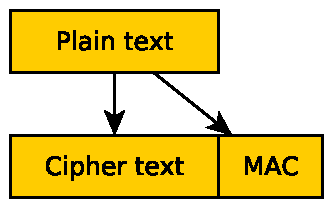
\includegraphics[width=0.9\textwidth]{images/encrypt-and-mac.pdf}
    \caption{Encrypt-and-MAC}
  \end{subfigure}
  \begin{subfigure}[b]{0.3\textwidth}
    \centering
    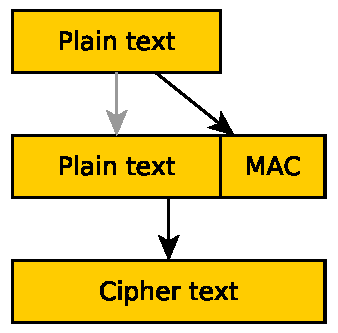
\includegraphics[width=0.9\textwidth]{images/mac-then-encrypt.pdf}
    \caption{MAC-then-encrypt}
  \end{subfigure}
  \begin{subfigure}[b]{0.3\textwidth}
    \centering
    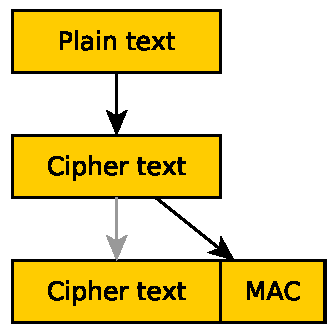
\includegraphics[width=0.9\textwidth]{images/encrypt-then-mac.pdf}
    \caption{Encrypt-then-MAC}
  \end{subfigure}
  \caption{Generic compositions of Authentized Encryption}
\end{figure}

\section{Competition for Authenticated Encryption: Security, Applicability and Robustness}

CAESAR is worldwide cryptographic competition, focused on finding new methods of authenticated encryption, that offer advantages against commonly used AES-GCM and will be suitable for widespread adoption. Submitted algorithms will be publicly evaluated by committee of researchers in fields of cryptography and cryptoanalysis.

\todo{popis algoritmů byly v soutěži, v čem se lišily, jaké a jak v nich byly nalezeny zranitelnosti a proto nepostoupily}

\todo{výběr algoritmu pro implementaci}

\subsection{Selection criteria}

\begin{description}
  \item[Online (one-pass)]
\end{description}



\subsection{NORX}

NO(T A)RX

ARX - Addition, Rotation, XOR

\subsubsection{Design goals}

\begin{itemize}
  \item \textbf{High security}
  \item \textbf{High speed} (in SW \textit{and} HW)
  \item \textbf{Simplicity} (of spec \textit{and} code)
  \item Online / one-pass
  \item Scalability (parallelism, unrolling)
  \item High key agility (no "key schedule")
  \item Side-channel leaks robustness (esp. timings)
\end{itemize}

\subsubsection{Parameters}

\begin{description}
  \item[Word Bit Size] $W \in {32, 64}$
  \item[Number of Rounds] $1 \leq R \leq 63$
  \item[Parallelism Degree] $0 \leq D \leq 255$ (0?)
  \item[Tag Bit Size] $|A| \leq 10W$
\end{description}

\begin{table}
  \centering
  \csvreader[
    after head=\begin{tabular}{llll}\toprule\csvlinetotablerow\\\midrule,
    late after line=\\,
    late after last line=\\\bottomrule\end{tabular}
  ]
    {tables/norx-proposed-instances.csv}{}
    {\texttt{\csvcoli} & \csvcolii & \csvcoliii & \csvcoliv}

  \caption{NORX proposed instances}
\end{table}

R=6: higher security margin

D=4: high throughput on parallel architectures

\subsection{Selection}

Benchmarks - Supercop, Brutus

\url{https://eprint.iacr.org/2014/850.pdf}
\url{http://www1.spms.ntu.edu.sg/~syllab/speed/}



